\section{Edge detection}
\paragraph*{Edges}
Edges correspond to areas in an image where there is a sharp change in intensity. These changes can occur due to:
\begin{itemize}
    \item Depth discontinuity
    \item Surface color discontinuity
    \item Illumination discontinuity
    \item Surface normal discontinuity
\end{itemize}
Edges hold the majority of the image information

\paragraph*{coordinates convention}
\begin{itemize}
    \item Origin top-left corner
    \item x: number of columns
    \item y: number of rows
\end{itemize}

\paragraph*{goal}: Extract info from the scene
\begin{itemize}
    \item Recognize objects
    \item geometry, viewpoint
\end{itemize}

\subsection{Image Gradient}
The gradient of an image is a measure of change in the intensity function. It points in the direction of the steepest increase in intensity. The gradient of an image is represented as:
\[
    \nabla f = \left( \frac{\partial f}{\partial x}, \frac{\partial f}{\partial y} \right)
\]
The magnitude of the gradient can be computed as:
\[
    |\nabla f| = \sqrt{\left( \frac{\partial f}{\partial x} \right)^2 + \left( \frac{\partial f}{\partial y} \right)^2}
\]
And the direction of the gradient is:
\[
    \theta = \tan^{-1}\left( \frac{\partial f}{\partial y} \middle/ \frac{\partial f}{\partial x} \right)
\]

Edges are perpendicular to the gradient direction, since it is the direction of steepest intensity change in the intensity funcition that rapresents the image.

\paragraph{Finite Difference Approximations}
To compute the gradient for a discrete digital image, we can use finite differences. The basic derivative approximations are:
\[
    \frac{\partial f}{\partial x} \approx f(x+1, y) - f(x, y)
\]
\[
    \frac{\partial f}{\partial y} \approx f(x, y+1) - f(x, y)
\]

\paragraph{Find the gradient using a filter}
Apply convolution with this filter
\[
    S_x = \begin{bmatrix}
        0 & 0  & 0 \\
        1 & -1 & 0 \\
        0 & 0  & 0
    \end{bmatrix}
    \quad
    S_y = \begin{bmatrix}
        0 & 1  & 0 \\
        0 & -1 & 0 \\
        0 & 0  & 0
    \end{bmatrix}
\]

\paragraph{The Sobel Operator}
The Sobel operator is a common method used to compute the image gradient. It applies a 3x3 convolution kernel to approximate the derivatives in the x and y directions:
\[
    S_x = \begin{bmatrix}
        1 & 0 & -1 \\
        2 & 0 & -2 \\
        1 & 0 & -1
    \end{bmatrix}
    \quad
    S_y = \begin{bmatrix}
        1  & 2  & 1  \\
        0  & 0  & 0  \\
        -1 & -2 & -1
    \end{bmatrix}
\]


\subsection*{What if the image is noisy?}:
In case of noise the image the gradient is influenced by all the sudden intensity changes and thus the edge cannot be detected.
\begin{figure}[H]
    \centering
    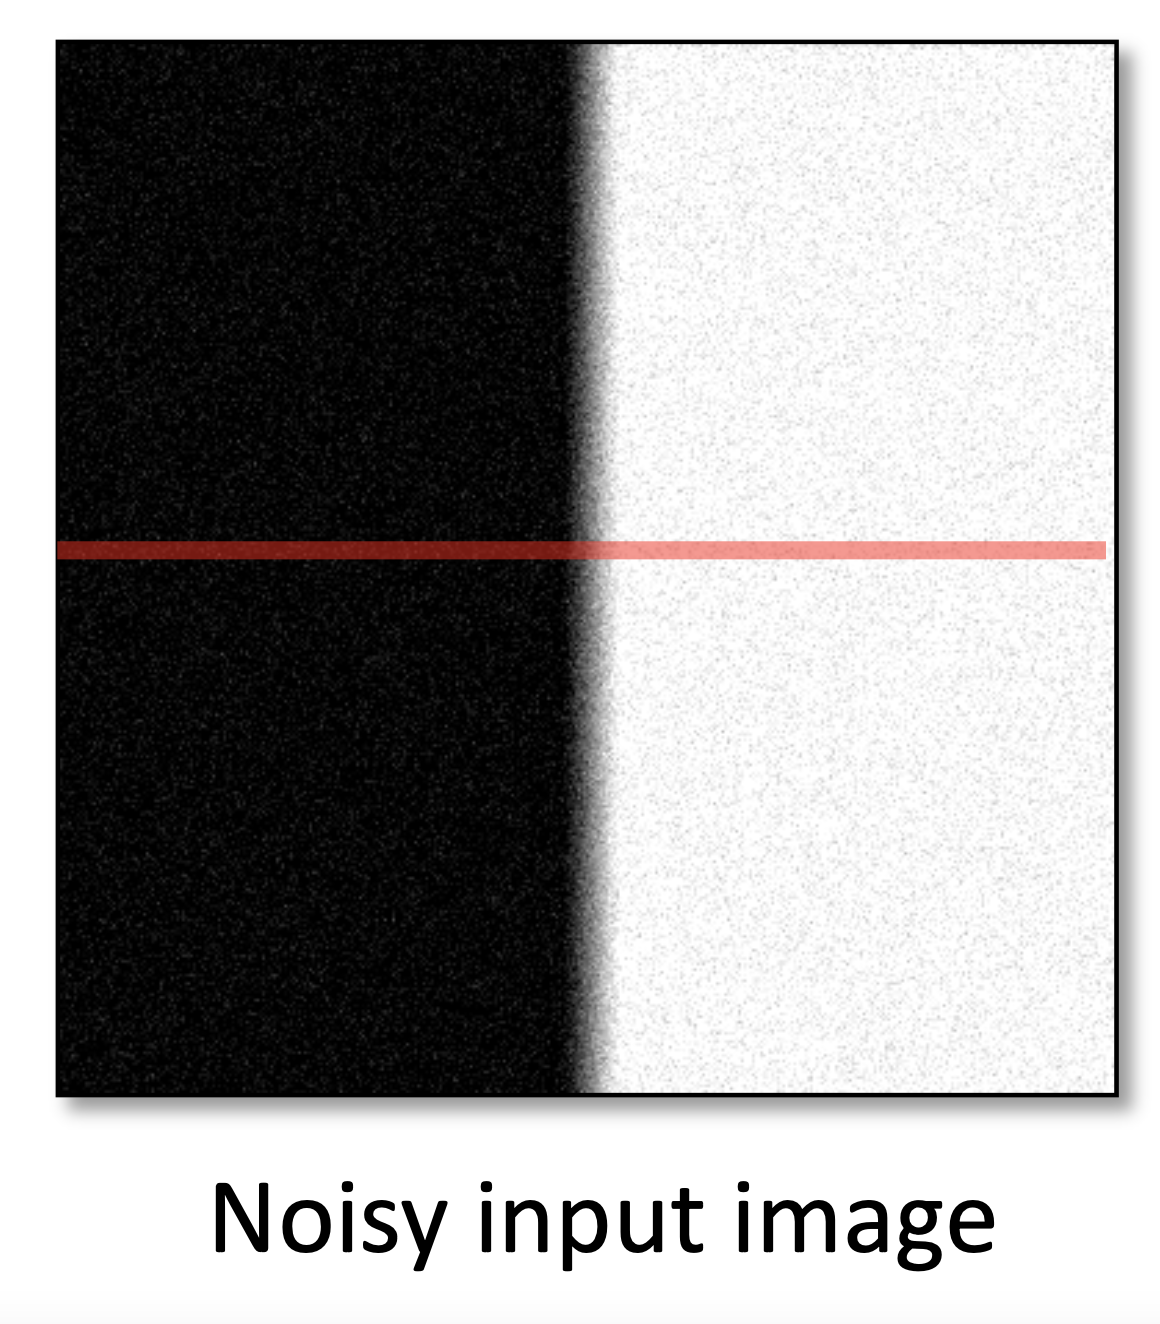
\includegraphics[width=0.5\linewidth]{Pictures/noisy_image.png}
\end{figure}

\begin{figure}[H]
    \centering
    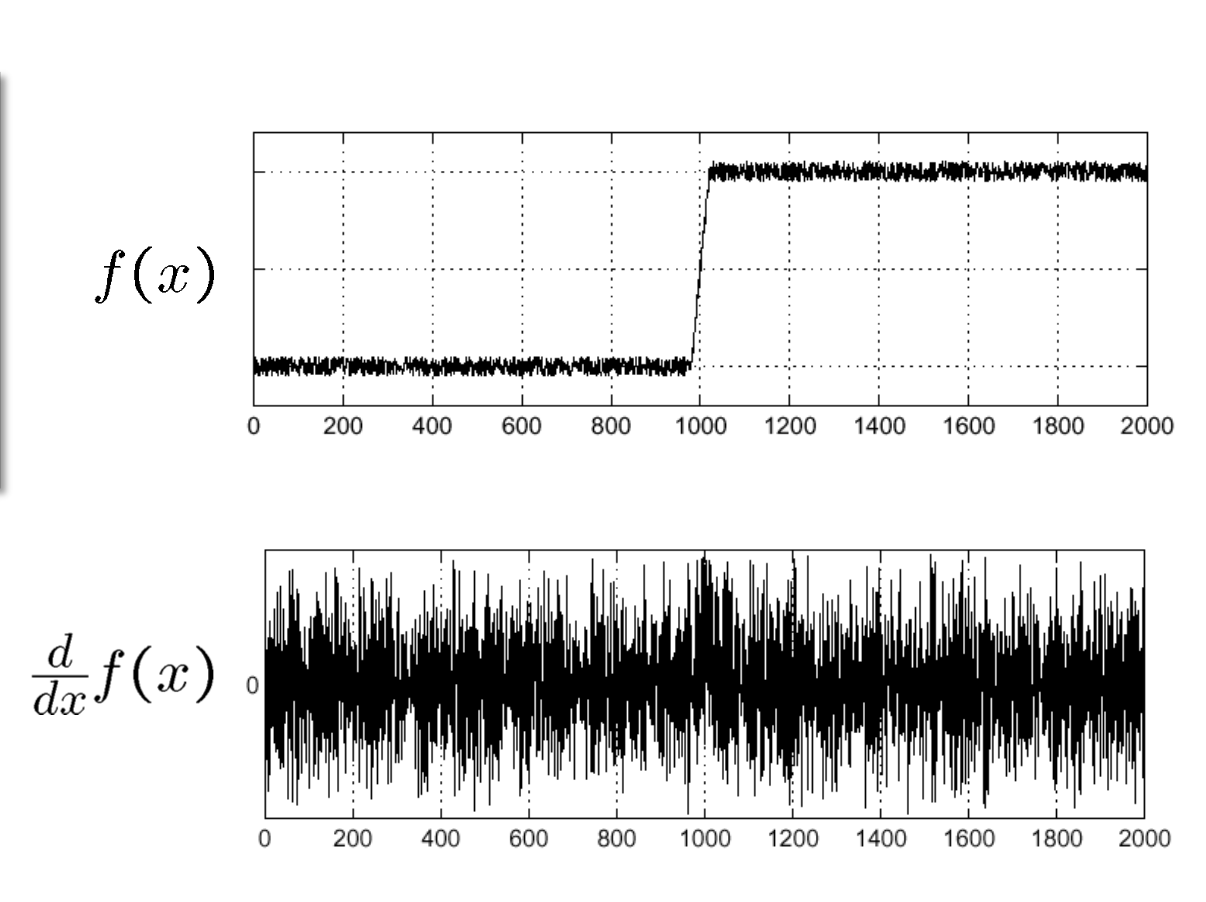
\includegraphics[width=0.6\linewidth]{Pictures/noisy_image_gradient.png}
    \caption{Noisy image gradient}
\end{figure}

If we apply smoothing with a Gaussian filter the





\begin{figure}[H]
    \centering
    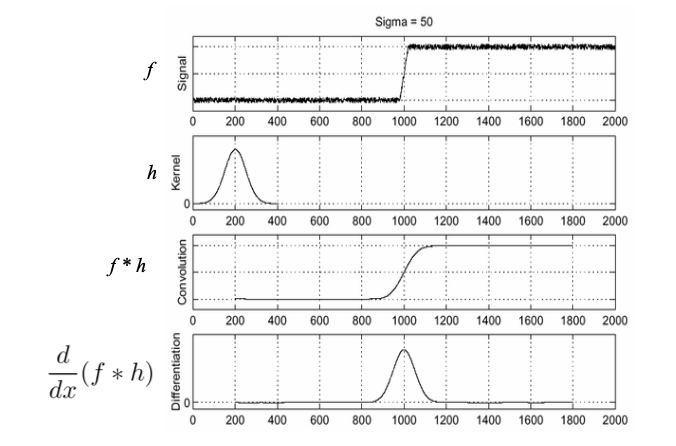
\includegraphics[width=0.6\linewidth]{Pictures/smoothing_and_gradient.png}
    \caption{Unite smoothing and gradient calculation}
    \label{fig:smoothing_and_gradient}
\end{figure}
\[
    \frac{d}{dx} (f * h) = f * \frac{d}{dx} h
\]



Can be united in a single step,
because this formula is true.





\paragraph*{NMS (Non Maximum gradient Suppression)}: For each pixel we find his neighbours
in the direction of the gradient. If the gradient doesn't point direcly to a pixel
we find the closest one to the direction.
Then we compare the magnitude of the pixel and his neighbours and we set to 0 the
smallest.

\section{Tradeoff Between Smoothing and Localization}
There is a tradeoff between noise reduction and edge localization. A larger Gaussian kernel reduces noise but blurs the edges, making them harder to localize accurately.

\section{Edge Detection}
Edge detection is a multi-step process:
\begin{enumerate}
    \item \textbf{Filtering:} First, the image is smoothed to reduce noise, typically using a Gaussian filter.
    \item \textbf{Enhancement:} Compute the image gradient to highlight the areas with large intensity changes.
    \item \textbf{Detection:} Identify locations where edges exist by finding the maxima in the gradient magnitude.
\end{enumerate}

\section{Canny Edge Detector}
The Canny edge detector is a popular edge detection algorithm that uses a multi-step process:
\begin{enumerate}
    \item \textbf{Gaussian Smoothing:} The image is smoothed with a Gaussian filter
          to reduce noise.
    \item \textbf{Gradient Calculation:} Compute the gradient intensity and direction
          for each pixel
    \item \textbf{Non-Maximum Suppression:} Suppress non-edge pixels by thinning
          multi-pixel wide edges to a single pixel width.
    \item \textbf{Hysteresis Thresholding:} Use two thresholds (high and low) to
          classify pixels as strong, weak, or non-edges. Strong edges are kept, weak
          edges are kept if they are connected to strong edges.
    \item \textbf{Edge Linking:} Connect edge pixels together to form continuous
          edges.
\end{enumerate}
